\chapter[Teoretická část studentské práce]{Teoretická část studentské\\ práce}

\section{Principy pořizování rentgenových snímků}
\label{sec:principy}
Pořizování rentgenových snímků je prováděno pomocí zdroje záření, rentgenovaného objektu a detektoru rentgenového záření. Rentgenové záření jsou elektromagnetické vlny s vlnovou délkou od \SI{10}{\nano\meter} do \SI{1}{\pico\meter} jejichž enerigie se nejčastěji pohybuje od \SI{1}{\kilo\eV} do \SI{200}{\kilo\eV}. \cite{AstroNuklFyzika-JadRadFyzika}

Jak již bylo zmíněno výše, scéna pro pořizování rentgenových snímků (\cref{fig:xray-scene}) se skládá ze zdroje rentgenového záření, rentgenovaného objektu a detektoru rentgenového záření. Zdroj rentgenového záření ozařuje elektromagnetickým vlněním o vlnové délce \SI{5}{\pico\meter} až \SI{50}{\pico\meter} rentgenovaný objekt. V závislosti na tloušťce a absorpčních vlastnostech objektu se část záření absorbuje a zbylá část záření dopadá na detektor rentgenového záření. Výstupem detektoru je poté obraz ve stupních šedi. \cite[kap.~3.2]{AstroNuklFyzika-JadRadMetody}

\begin{figure}[bh]
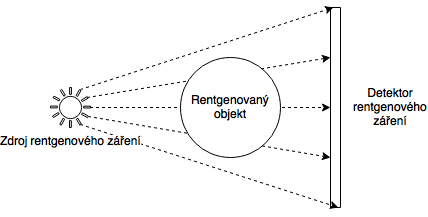
\includegraphics[width=\textwidth]{xray-scene}
\caption{Scéna pro pořizování rentgenových snímků.}
\label{fig:xray-scene}
\centering
\end{figure}

\subsection{Vznik rentgenového záření}
\label{sec:vznik-rentgenoveho-zareni}
Elektromagnetické záření, kterému se říká rentgenové záření vzniká buď při přechodu elektronů mezi vnitřními vrstvami těžších atomů -- charakteristické X-záření, nebo při dopadu a prudkém zabrzdění elektronů -- brzdné záření. \cite{AstroNuklFyzika-JadRadFyzika}

\subsubsection{Brzdné záření}
V případě, že se akcelerovaný elektron přiblíží k jádru atomu silné Coulombovy síly mezi jádrem atomu a letícím elektronem způsobí silné zbrzdění elektronu a změnu jeho trajektorie. Během zbrzdění rychle letícího elektronu  je jeho kinetická energie přeměňována na brzdné záření. \cite[str.~89]{Diagnostic-Radiology-Physics} Tento proces popisuje \cref{fig:bremsstrahlung-xray}.

\begin{figure}[bh]
\centering
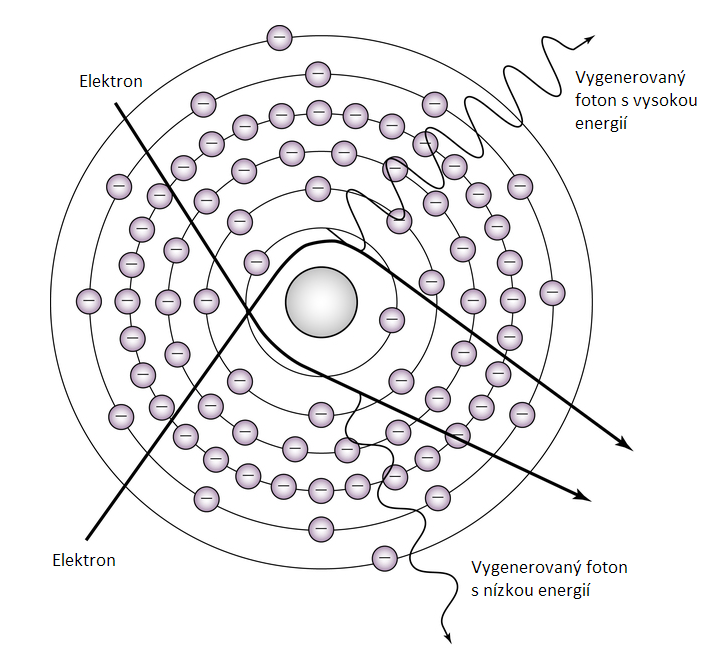
\includegraphics[width=0.75\textwidth]{bremsstrahlung-xray}
\caption{Vznik brzdného záření při interakci rychle se pohybujícího elektronu s atomem wolframu. \cite{the-xray-beam}}
\label{fig:bremsstrahlung-xray}
\end{figure}

Ideální spektrum brzdného záření lze popsat pomocí zjednodušeného modelu, který neuvažuje kvantovou mechaniku. Zjednodušený model uvažuje proud elektronů přibližující se k atomu. Uvážíme-li pole v okolí jádra atomu rozdělené na několik kruhových vrstev dle působících brzdných sil, generované brzdné záření brzděním proudu elektronů má spektrum, které odpovídá plochám těchto vrstev. Čím blíže je vrstva pole k jádru atomu, tím větší brzdnou sílou působí na letící elektron a tím větší je energie vygenerovaného fotonu. Zároveň čím je vrstva pole vzdálenější od jádra atomu, tím větší má plochu a tím více fotonů je schopna vygenerovat. Fotony generované ve vzdálenějších vrstvách mají nižší energii vzhledem k nižším brzdným silám působících na přibližující se elektrony. \cite[kap.~THE~X-RAY TUBE]{The-Physical-Principles-of-Medical-Imaging}

Ideální spektrum brzdného záření zjednodušeného modelu ukazuje \cref{fig:bremsstrahlung-xray-char}. Ze spektra je zřetelné, že největší energii, která se blíží kinetické energii elektronů má jen zlomek z celkového počtu generovaných fotonů (fotony generované elektrony, které byly zabrzděny ve vrstvě nejblíže jádru).

\begin{figure}[bh]
\centering
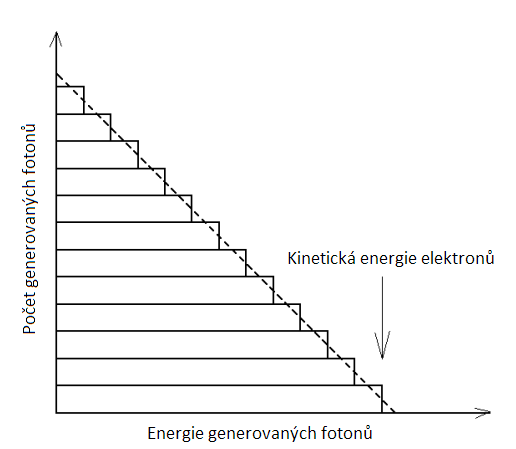
\includegraphics[width=0.75\textwidth]{bremsstrahlung-xray-char}
\caption{Ideální spektrum brzdného záření. \cite[str.~90]{Diagnostic-Radiology-Physics}}
\label{fig:bremsstrahlung-xray-char}
\end{figure}

\subsubsection{Charakteristické záření}
Charakteristické záření vzniká při přechodu atomového elektronu z vyšší vrstvy do nižší. Při přechodu elektron ztrácí energii, která je emitovaná jako foton charakteristického záření. Energie emitovaného fotonu odpovídá rozdílu energií vrstev mezi kterými elektron přechází. Spektrum charakteristického záření je monochromatické a odvíjí se od druhu atomu. Proces vzniku charakteristického záření popisuje \cref{fig:characteristic-xray}. \cite[str.~91]{Diagnostic-Radiology-Physics}

\begin{figure}[h]
\centering
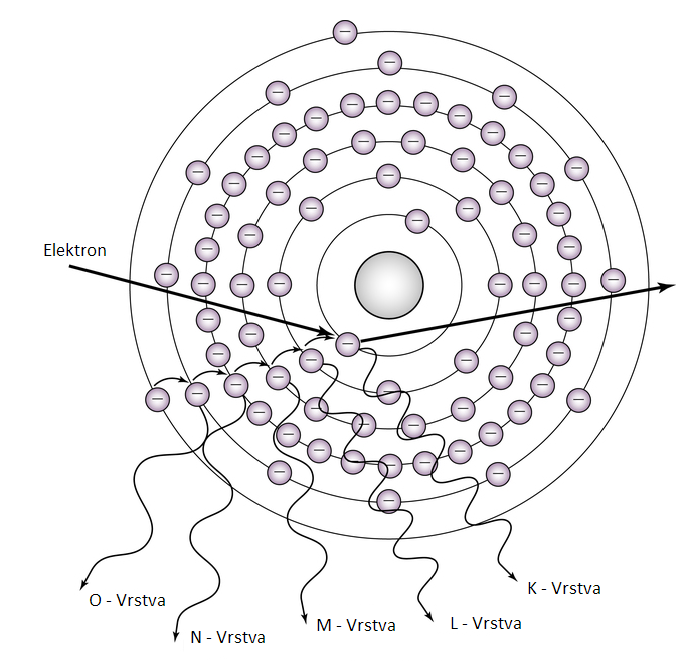
\includegraphics[width=0.75\textwidth]{characteristic-xray}
\caption{Vznik charakteristického záření v atomu wolframu při vyražení elektronu z K-Vrstvy elektronem s kinetickou energií vyšší, než vazební energie vyraženého elektronu. \cite{the-xray-beam}}
\label{fig:characteristic-xray}
\end{figure}

\subsection{Rentgenka}
Zdrojem rentgenového záření při pořizování rentgenových snímků je nejčastěji speciální vakuová elektronka (\cref{fig:xray-tube}), které je často nazývána jako rentgenka, rentgenová lampa či rentgenová trubice. \cite{AstroNuklFyzika-JadRadMetody} Rentgenku si lze představit, jako zařízení, které převádí energii elektronů na elektromagnetické záření s odpovídající energií. Expozice a spektrum záření může být řízena nastavením parametrů rentgenky jako jsou napětí (\SI{}{\kV}), proud (\SI{}{\mA}) a doba expozice (\SI{}{\s}). \cite[str.~93]{Diagnostic-Radiology-Physics}

\subsubsection{Principy fungování rentgenky}
Energie, která je přeměňována v rentgence na rentgenové záření a teplo je do rentgenky přiváděna proudem elektronů s potenciální energií odpovídající napětí na vysokonapěťovém zdroji (\SI{1}{\kV} odpovídá \SI{1}{\k\eV}). 
Během průchodu elektronu rentgenkou dochází k přeměně jeho potenciální energie na energii kinetickou, která je následně přeměněna na elektromagnetické záření a teplo. 

Kinetická energie elektronu při dopadu na anodu odpovídá napětí na vysokonapěťovám zdroji, tedy původní potenciální energii. Kinetická energie je přeměňována zbrzdění atomů při dopadu na anodu  při interakci s atomy materiálu na brzdné a charakteristické rentgenové záření. \cite[kap.~ELECTRON ENERGY]{The-Physical-Principles-of-Medical-Imaging}
Proud elektronu je emitován při žhavení katody se záporním napětí. Množství emitovaných elektronů může být řízeno změnou proudu žhavení, tedy změnou teploty žhaveného vlákna. \cite[str.~93]{Diagnostic-Radiology-Physics} 

\paragraph{Spektrum rentgenového záření rentgenky}
popisuje \cref{fig:xray-spectre}. Při dopadu elektronů na anodu vznikají dva typy rentgenového záření--brzdné a charakteristické, jejichž obecné principy byly popsány v kapitole \ref{sec:vznik-rentgenoveho-zareni}. Obrázek ukazuje celkem tři charakteristiky záření při napětí na elektrodách \SI{90}{\kV}:
\begin{enumerate}[label=(\alph*)]
\item Ideální spektrum brzdného brzdného záření--spektrum, které již bylo popsáno v obrázku \ref{fig:bremsstrahlung-xray-char}.
\item Generované spektrum--reálné spektrum skládající se z brzdného a charakteristického záření.
\item Filtrované spektrum--spektrum s útlumem dopovídajícím \SI{2.5}{\mm}Al.
\end{enumerate}

\begin{figure}[hb]
\centering
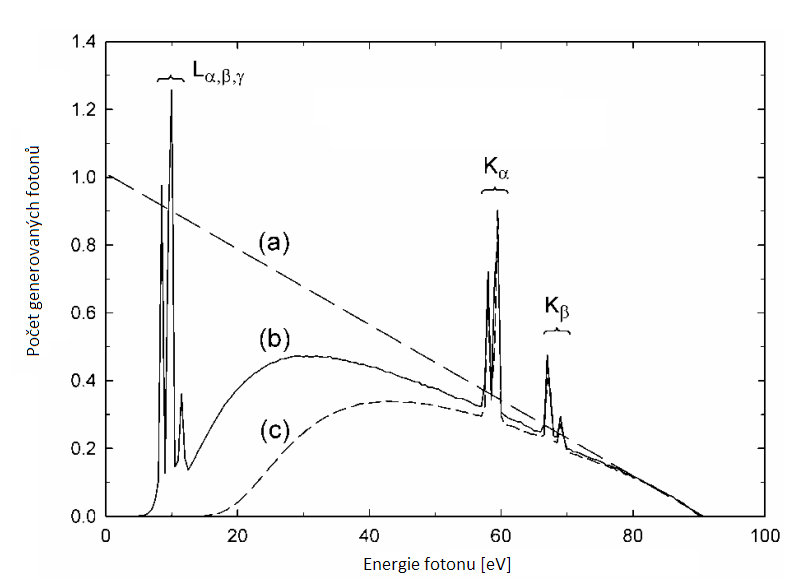
\includegraphics[width=\textwidth]{xray-spectre}
\caption{Rentgenka se zdroji proudu a napětí. \cite[str. 93]{Diagnostic-Radiology-Physics}}
\label{fig:xray-spectre}
\end{figure}

\subsubsection{Konstrukce rentgenky}
Z důvodu tepelného ohřevu anody po dopadu zrychlených elektronů a vysokého napětí na elektrodách musí být rentgenky oproti běžným elektronkám robustní konstrukce. Chlazení samotné anody je zajištěno její velikostí a také rotací  nebo aktivním chlazením. Rentgenky lze rozdělit kategorií podle způsobu využití a konstrukce \cite[kap. 3.2]{AstroNuklFyzika-JadRadMetody}:
\begin{itemize}
\item Rentgenky pro průmyslové ozařování a radioterapeutické použití - rentgenky s pevnou anodou, kde je chlazení zajištěno průtokem chladícího média. U toho typu rentgenek je častým požadavkem vysoká energie a intenzita záření. Naopak zde není potřebné zaměřování elektronů do téměř bodového ohniska. 
\item Rentgenky pro rentgenovou diagnostiku - rentgenky se soustředěním elektronů do ohniska. U tohoto typu rentgenek se využívá rotující anody proti nadměrnému přehřívání anody v místě ohniska.
\item Speciální rentgenky - rentgenky rozšířené o třetí elektrodu (drátěnou mřížku umístěnou mezi katodou a anodou v těsné blízkosti katody) sloužící k řízení proudu protékajícího anodou. Proud je řízen napětím, které je přivedeno na drátěnou mřížku.
\end{itemize}

Generované záření ještě před tím, než opustí rentgenku musí projít skrz různé materiály, které záření filtrují. Těmito materiály mohou být například samotná anoda, materiál trubice rentgenky, chladící medium apod. Úbytek záření při průchodu těmito materiály se uvádí jako útlum ekvivalentní k \SI{1}{\mm}Al--jednomu milimetru hliníku. Typická hodnota útlumu u běžných rentgenek bývá od \SI{0.5}{\mm}Al do \SI{1}{\mm}Al. 

\begin{figure}[hb]
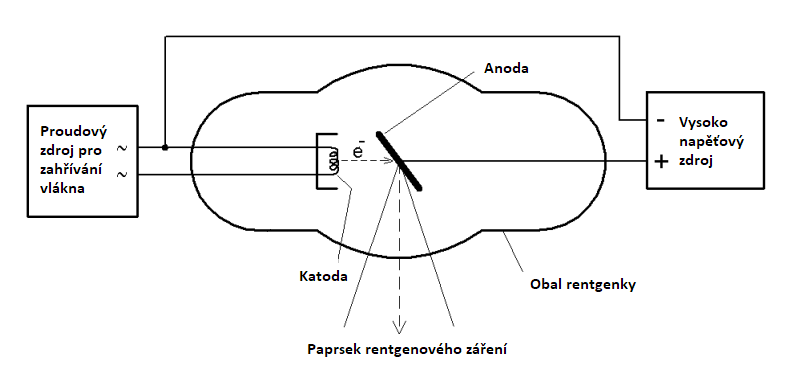
\includegraphics[width=\textwidth]{xray-tube}
\caption{Rentgenka se zdroji proudu a napětí. \cite[str. 93]{Diagnostic-Radiology-Physics}}
\label{fig:xray-tube}
\centering
\end{figure}

\paragraph{Anoda}
je součást rentgenky, kde je generováno rentgenové záření. Anoda bývá tvořena relativně velikým kusem železného materiálu, na který je přivedeno kladné napětí vysokonapěťového zdroje. Anoda jako taková plní v rentgence dvě funkce:
\begin{itemize}
\item Převod elektrické energie na rentgenové záření.
\item Odvod tepla, které vzniká během procesu generování rentgenového záření.
\end{itemize}
Jako vhodný materiál anody lze považovat materiál, který dokáže co největší podíl elektrické energie převést na záření, čili materiál, který má vysokou efektivitu převodu (jak již bylo zmíněno přebytečná energie je přeměňována na teplo). Efektivita převodu elektrické energie na záření závisí na atomovému číslu materiálu anody (Z) a kinetické energii dopadajícího elektronu na katodu.\cite{The-Physical-Principles-of-Medical-Imaging}

Nejvíce rentgenek využívá jako materiál anody wolfram s atomovým číslem 74. Wolfram je vhodný díky vysokému atomovému číslu a vysokému bodu tání. V některých případech je využíváno slitiny wolframu a rhenia, která je však využívána pouze jako povrchový materiál. Zbylá část anody anody poté bývá vyrobena z relativně lehkého materiálu, který má dobré tepelné vlastnosti. Těmito materiály mohou být například molybden nebo grafit. Výjimkou jsou anody rentgenek pro mamografii, kdy je využíváno molybdenu jako materiálu pro povrch anody.\cite{The-Physical-Principles-of-Medical-Imaging}

Anody lze dělit v závislosti na výkonu rentgenky (\cref{fig:anodes}). Pro aplikace, kdy není potřebná vysoká energie rentgenového záření je využíváno statických anod. Tato anoda se skládá z wolframu, který je usazen v měděném bloku, který slouží k odvádění tepla. Tento typ anod se využívá například dentistických nebo přenosných rentgenkách. Druhým typem anod jsou rotační anody. Anoda je připojená k rotoru asynchronního motoru, který je umístěn přímo ve vakuové trubici rentgenky. Vinutí statoru je naopak umístěno vně rentgenkové trubice. Samotná anoda má kruhový tvar v podobě terče se skosenými hranami na okrajích. Paprsek elektronů poté dopadá na zkosenou hranu, která je otáčena rotorem, tudíž je anoda tepelně namáhána rovnoměrně podél celého obvodu, což umožňuje generovat záření s vyšší energií. \cite[str.~98]{Diagnostic-Radiology-Physics}

\begin{figure}[hb]
\centering
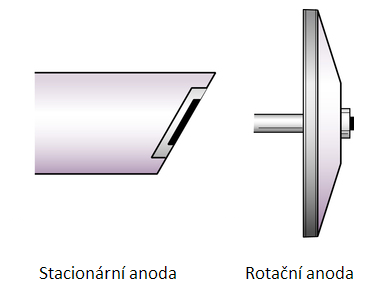
\includegraphics{anodes}
\caption{Rotační a stacionární anoda. \cite{the-xray-beam}}
\label{fig:anodes}
\end{figure}


\paragraph{Katoda}
je druhou elektrodou rentgenky, která má za úkol generování paprsku elektronů pomocí žhavícího vlákna (\cref{fig:cathode}). Katoda je připojena a záporné napětí vysokonapěťového zdroje a zároveň k střídavému zdroji proudu, který slouží k žhavení vlákna katody a tím i emitování elektronů.\cite[str.~93]{Diagnostic-Radiology-Physics} Velikost žhavícího vlákna ovlivňuje velikost ohniska paprsku elektronů na anodě. Čím větší je žhavící vlákno tím větší ohnisko je.

\begin{figure}[hb]
\centering
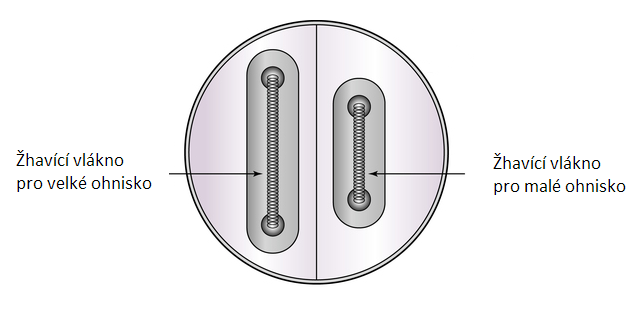
\includegraphics{cathode}
\caption{Katoda s dvěmi žhavícími vlákny. \cite{the-xray-beam}}
\label{fig:cathode}
\end{figure}

\subsection{Detekce rentgenového záření}
\subsubsection{Filmové systémy}
Pro získávání snímků pomocí filmu je využíváno filmových systému. Tento systém využívá filmu, který je citlivý na světelné záření. Pro získání rentgenového snímku je třeba vložit film do rentgenového zařízení a poté film vyvolat. Film bývá vložen do plastové kazety, uvnitř kterých je fosforová vrstva, která přeměňuje rentgenové záření na světelné záření, které lze detekovat filmem vloženým do kazety. Výhodou filmových systémů je, že film jako takový má vysokou citlivost a zároveň se při detekci na rozdíl od digitálních systémů neztrácí žádná viditelná informace. \cite[str.~155]{Diagnostic-Radiology-Physics} Filmové systémy jsou využívány jak ve zdravotnictví, tak v průmyslu, nicméně jejich využití je spíše na ústupu. Vzhledem k povaze této práce se jimi práce nebude více zabývat.

\subsection{Digitální systémy}
Čím dál častěji filmové systémy nahrazují systémy digitální. tyto systémy lze rozdělit do dvou kategorií na systémy pro nepřímou radiografii -- Computed Radiography (\zk{zk:CR}) a přímou radiografii -- Direct Radiography  (\zk{zk:DR}). \zk{zk:CR} vychází z klasických filmových systému u kterých je místo filmu využíváno speciálních fosforových fólií. Proces digitalizace je pak prováděn ve speciálním zařízení.
\zk{zk:DR} na rozdíl od \zk{zk:CR} převádí záření na digitální snímek přímo, nicméně samotný proces převodu může být přímý (záření je převáděno snímači na elektrickou veličinu) nebo nepřímý (záření je nejprve převedeno na světelné záření, které je poté převáděno na elektrickou veličinu). \cite[str.~676]{Advances-in-Digital-Radiography}

\subsubsection{Nepřímá radiografie (\zk{zk:CR})}
Jak již bylo zmíněno výše, \zk{zk:CR} využívá technologie, která je velice podobná filmovým systémům. Paměťové fólie jsou tvořeny citlivou vrstvou tvořenou fosforovými krystaly. \cite[str.~676]{Advances-in-Digital-Radiography}. 

Proces ukládání informace a její digitalizaci popisuje \cref{fig:cr}. Energie dopadajícího záření je absorbována a dočasně (řádově několik hodin) uložena v paměťové fólii přechodem elektronů atomů fosforových krystalů do vyšších energických hladin (metastabilních). Digitalizace uložené energie ve fólii poté probíhá v zařízení, které dokáže pomocí laserového paprsku uvolňovat elektrony z metastabilních hladin do vodivostního pásu. Při uvolňování elektronů dochází k emitování světelného záření, které je poté možné měřit fotonásobičem připojeným na AD převodník. \cite[str.~677]{Advances-in-Digital-Radiography}. Výhodou tohoto systému je snadná integrace do stávajících filmových systémů. Nevýhodou může být vysoká časová náročnost vyvolávání snímků, nízké prostorové rozlišení. \cite[str~209]{Diagnostic-Radiology}

\begin{figure}[ht]
\centering
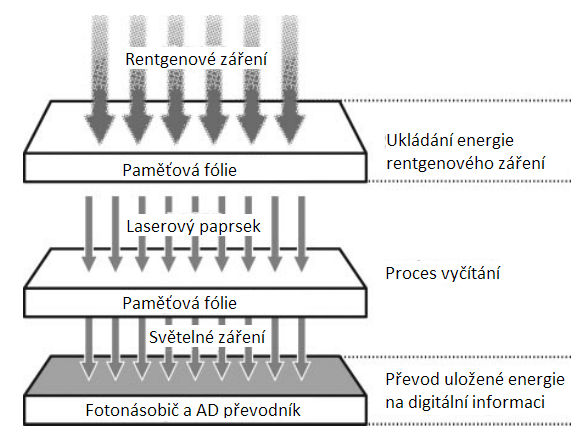
\includegraphics{cr}
\caption{Proces získání digitálního snímku při nepřímé radiografii. \cite[str.~677]{Advances-in-Digital-Radiography}}
\label{fig:cr}
\end{figure}

\subsubsection{Přímá radiografie (\zk{zk:DR})}
V případě, že jsou snímky snímány přímo, jedná se o \zk{zk:DR}. \zk{zk:DR} je možné dále dělit podle způsobu převodu rentgenového řazení na \zk{zk:DR} s přímým  převodem a \zk{zk:DR} s nepřímým převodem. Při přímém převodu je rentgenové záření snímáno přímo, naopak při nepřímém převodu je záření převáděno zpravidla pomocí scintilační vrstvy na záření světelné, které je poté snímáno fotocitlivými snímači. Rozdíl mezi přímým a nepřímým převodem rentgenového záření popisuje obrázek \cref{fig:direct-indirect-tft}.

\begin{figure}[ht]
\centering
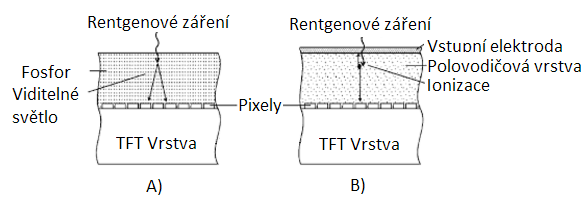
\includegraphics{direct-indirect-tft}
\caption{Polovodičový TFT detektor s nepřímým (A) a přímým (B) převodem rentgenového záření \cite[str.~511]{Radiation-Detection-and-Measurement}}
\label{fig:direct-indirect-tft}
\end{figure}

\paragraph{DR s přímým převodem}
využívají polovodičové vrstvy ze selenu (Se), který dokáže převádět fotony rentgneového záření na elektrickou energii. \zk{zk:DR} systémy s přímým převodem mohou využívat buď selenové foto-válce s AD převodníkem nebo selenové polovodičové vrstvy spojené s vrstvou tenkovrstvých tranzistorů -- Thin Film Tranzistors (\zk{zk:TFT}). \cite[str.~678]{Advances-in-Digital-Radiography} Výhodou těchto systémů je především vysoké prostorové rozlišení. Díky nízkému atomovéu číslu selenu je u těchto detektorů poměrně nízká absorpce rentgenového záření. Díky tomuto faktu je systémů s přímým převode využíváno spíše v mamografii. \cite[str~210]{Diagnostic-Radiology}

Systémy, které využívají foto-válců otáčí samotným válcem, na který dopadá rentgenové záření, které se přeměňuje na náboj na povrchu válce. Náboj na povrchu otáčejícího se válce je poté vyčítán pomocí AD převodníku. \cite[str.~677]{Advances-in-Digital-Radiography}. Tento princip je založen na stejném principu jako foto válec laserových tiskáren.
 
Na podobné principu pracují systémy s vrstvou \zk{zk:TFT} (\cref{fig:direct-tft}). Matice \zk{zk:TFT} ukládá generovaných náboj do paměťových kondenzátorů, jejichž napětí může být vyčítáno AD převodníkem. Takovýto detektor se skládá z elektrody na kterou je přivedeno vysoké kladné napětí, polovodičové vrstvy selenu a vrstvy \zk{zk:TFT} kondenzátory pro ukládání náboje generovaného rentgenovým záření. Rentgenové záření generuje v selenové vrstvě elektrony a díry. Díky tomu vzniká v polovodiči náboj, který je přímo úměrný rentgenovému rentgenovému záření. Tento náboj je poté díky silnému elektrickému poli odváděn do kondenzátorů v \zk{zk:TFT} vrstvě. Napětí kondenzátoru může být poté vyčteno přivedení záporného napětí na gate příslušného tranzistoru.

\begin{figure}[ht]
\centering
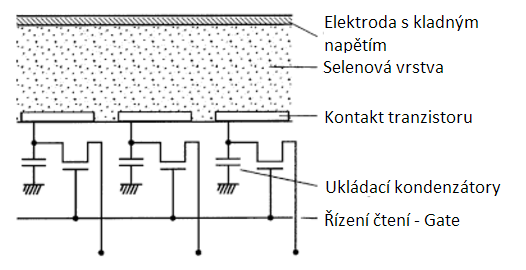
\includegraphics{direct-tft}
\caption{Princip polovodičového TFT detektoru s přímým převodem rentgenového záření \cite[str.~511]{Radiation-Detection-and-Measurement}}
\label{fig:direct-tft}
\end{figure}

\paragraph{DR s nepřímým převodem}
využívá scintilační vrstvy k převodu rentgenového záření na světelné záření, které je poté snímáno dalšími vrstvami. Scintilační vrstvy můžou být jak strukturované, tak nestrukturované. V případě nestrukturované scintilační vrstvy generované světelné záření přirozeně dopadá na přilehlé snímače světelného záření, které odpovídají jednotlivým pixelům. Naopak v případě strukturované scintilační vrstvy světelné záření díky speciální struktuře vrstvy dopadá pouze na jeden snímač světelného záření. Díky tomu je zajištěno lepší prostorové rozlišení detektoru. Rozdíly mezi strukturovanou a nestrukturovanou scintilační vrstvou popisuje \cref{fig:structured-unstructured-scintillator}.

\begin{figure}[ht]
\centering
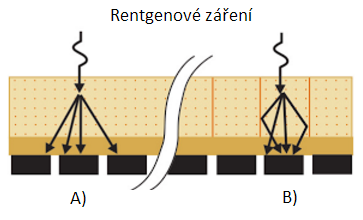
\includegraphics{structured-unstructured-scintillator}
\caption{Rozdíl mezi nesturkturovanou (A) a strukturovanou (B) scintilační vrstvou TFT detektoru s nepřímým převodem. \cite[str~210]{Diagnostic-Radiology}}
\label{fig:structured-unstructured-scintillator}
\end{figure}

V případě, že je jako detekční vrstva využíváno \zk{zk:TFT} matice, musí být pod scintilační vrstvu přidána vrstva detekující světelné záření. Taková vrstva je nejčastěji tvořena foto-diodovým polem. Elektrická energie generována foto-diodovým polem je poté ukládána pomocí kondenzátorů \zk{zk:TFT} matice a následně  čtena AD převodníkem.

Detekční vrstva může být také realizována pomocí \zkratka{zk:CCD}. V tomto případě je pomocí \zk{zk:CCD} detektorů přímo detekováno viditelné světlo, které je generováno v scintilační vrstvě. Díky poměrně malé velikosti \zk{zk:CCD} snímačů je nutné snímače kombinovat, případně využívat čoček.

